% Requires in the main document preamble:
% \usepackage{tikz}
% \usetikzlibrary{positioning,calc}

\begingroup
\definecolor{stackfill}{HTML}{F8FAFC}
\definecolor{stackborder}{HTML}{475569}
\definecolor{stackarrow}{HTML}{64748B}
\definecolor{stacktext}{HTML}{1E293B}
\definecolor{subfill}{HTML}{F1F5F9}

% Technology badge colors
\definecolor{htmlcol}{HTML}{E34F26}
\definecolor{csscol}{HTML}{1572B6}
\definecolor{jscol}{HTML}{F7DF1E}
\definecolor{jinjacol}{HTML}{111111}
\definecolor{metamaskcol}{HTML}{F6851B}
\definecolor{etherscol}{HTML}{627EEA}
\definecolor{pythoncol}{HTML}{3776AB}
\definecolor{groqcol}{HTML}{111111}
\definecolor{llmcol}{HTML}{4B5563}
\definecolor{cyphercol}{HTML}{2563EB}
\definecolor{neo4jcol}{HTML}{008CC1}
\definecolor{nodecol}{HTML}{339933}
\definecolor{zerodevcol}{HTML}{2563EB}
\definecolor{viemcol}{HTML}{627EEA}
\definecolor{ethcol}{HTML}{627EEA}

% Human-made colored badge
\newcommand{\techbadge}[3]{%
\tikz[baseline=-0.65ex]{
    \node[
        draw=#1,
        fill=#1,
        rounded corners=1.4pt,
        text=white,
        font=\sffamily\bfseries\tiny,
        inner xsep=3.6pt,
        inner ysep=1.9pt
    ] {#2};
}%
\hspace{0.35em}#3%
}

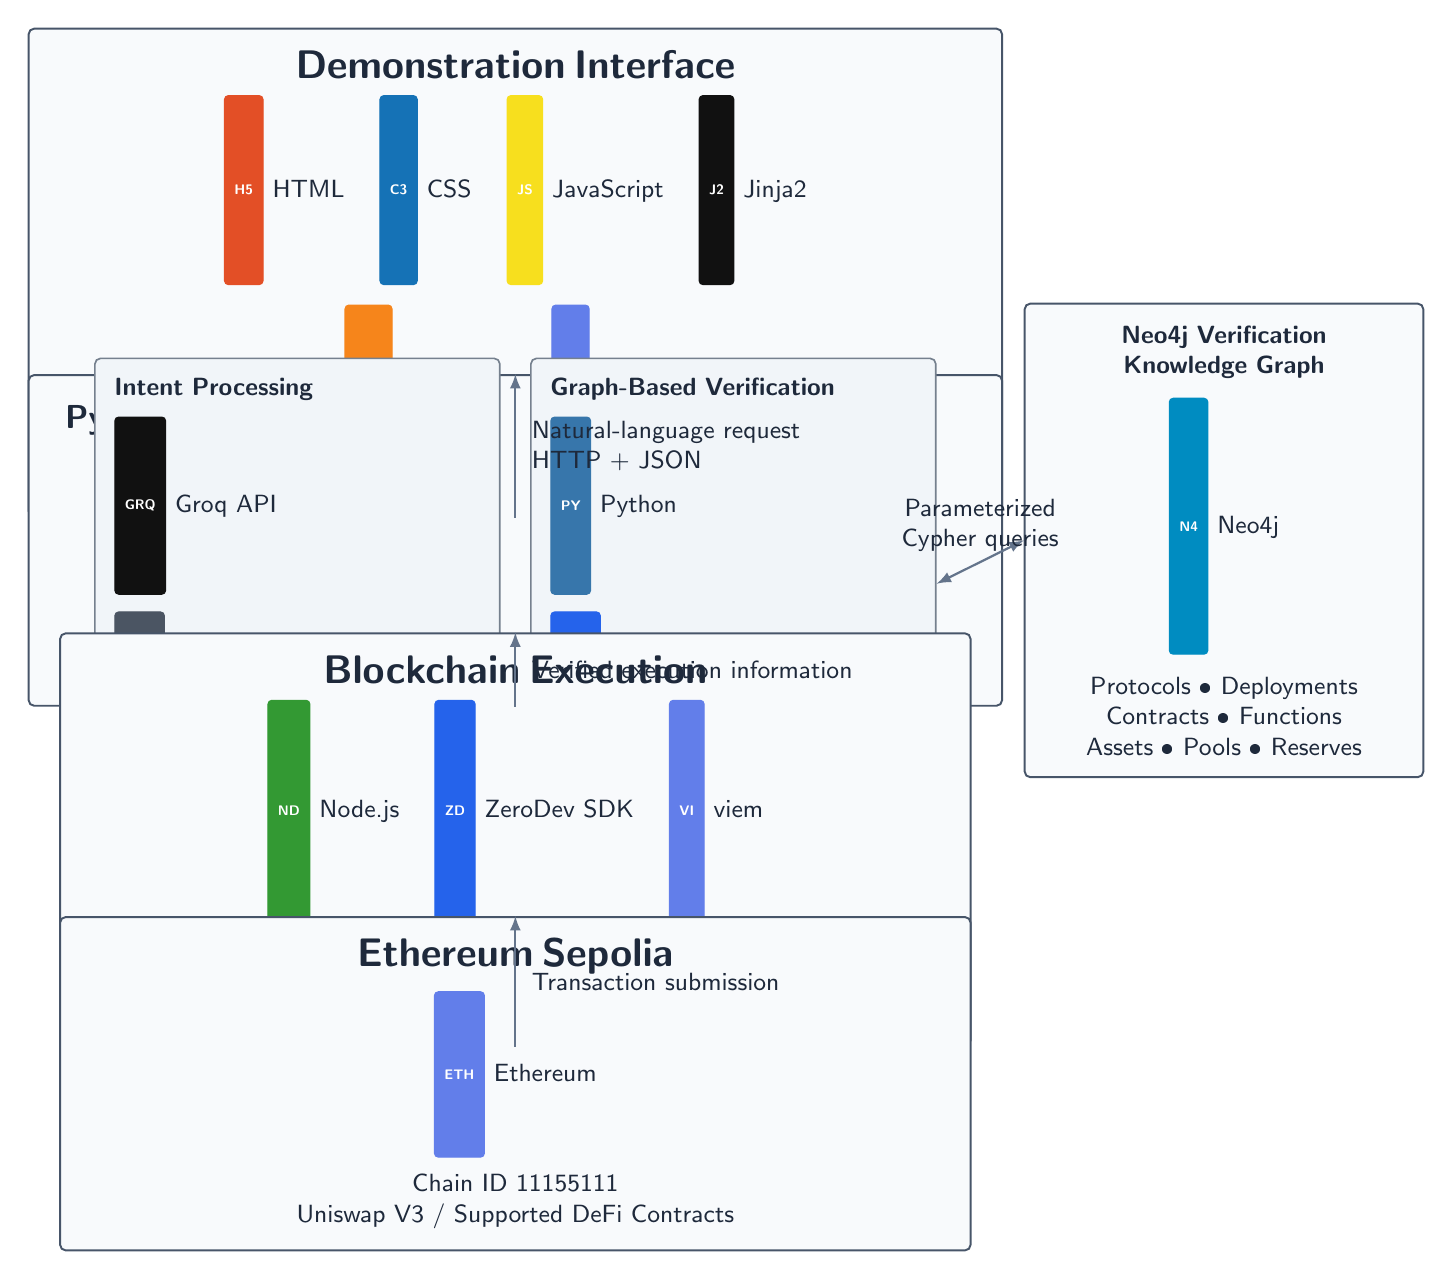
\begin{tikzpicture}[
    font=\sffamily\small,
    >=latex,
    outerbox/.style={
        draw=stackborder,
        fill=stackfill,
        rounded corners=2pt,
        line width=0.7pt,
        text=stacktext,
        align=center,
        inner sep=8pt
    },
    backendbox/.style={
        draw=stackborder,
        fill=stackfill,
        rounded corners=2pt,
        line width=0.7pt,
        text=stacktext,
        align=center,
        inner sep=8pt
    },
    subbox/.style={
        draw=stackborder!75,
        fill=subfill,
        rounded corners=2pt,
        line width=0.6pt,
        text=stacktext,
        align=left,
        inner sep=7pt
    },
    flow/.style={
        ->,
        draw=stackarrow,
        line width=0.8pt
    },
    sideflow/.style={
        <->,
        draw=stackarrow,
        line width=0.8pt
    }
]

% ------------------------------------------------------------------
% Main nodes
% ------------------------------------------------------------------

% Demonstration interface
\node[
    outerbox,
    text width=11.8cm,
    minimum height=2.4cm
] (ui) at (0,0) {%
    {\bfseries\Large Demonstration Interface}\\[5pt]
    \techbadge{htmlcol}{H5}{HTML}
    \hspace{0.7em}
    \techbadge{csscol}{C3}{CSS}
    \hspace{0.7em}
    \techbadge{jscol}{JS}{JavaScript}
    \hspace{0.7em}
    \techbadge{jinjacol}{J2}{Jinja2}\\[6pt]
    \techbadge{metamaskcol}{MM}{MetaMask}
    \hspace{0.8em}
    \techbadge{etherscol}{ES}{ethers.js}
};

% Backend container
\node[
    backendbox,
    text width=11.8cm,
    minimum height=4.2cm
] (backend) at (0,-3.4) {};

\node[
    anchor=north west,
    text=stacktext,
    font=\sffamily\bfseries\large
] at ([xshift=0.35cm,yshift=-0.28cm]backend.north west)
{Python Backend --- FastAPI};

% Inner backend boxes
\node[
    subbox,
    text width=4.65cm,
    minimum height=2.25cm,
    anchor=west
] (intent) at ([xshift=-5.35cm,yshift=-0.55cm]backend.center) {%
    {\bfseries Intent Processing}\\[5pt]
    \techbadge{groqcol}{GRQ}{Groq API}\\[5pt]
    \techbadge{llmcol}{LLM}{\texttt{openai/gpt-oss-20b}}
};

\node[
    subbox,
    text width=4.65cm,
    minimum height=2.25cm,
    anchor=east
] (verify) at ([xshift=5.35cm,yshift=-0.55cm]backend.center) {%
    {\bfseries Graph-Based Verification}\\[5pt]
    \techbadge{pythoncol}{PY}{Python}\\[5pt]
    \techbadge{cyphercol}{CYP}{Cypher queries}
};

% Neo4j box
\node[
    outerbox,
    text width=4.5cm,
    minimum height=3.25cm
] (neo4j) at (9.0,-3.4) {%
    {\bfseries Neo4j Verification\\Knowledge Graph}\\[6pt]
    \techbadge{neo4jcol}{N4}{Neo4j}\\[7pt]
    Protocols \textbullet\ Deployments\\
    Contracts \textbullet\ Functions\\
    Assets \textbullet\ Pools \textbullet\ Reserves
};

% Execution
\node[
    outerbox,
    text width=11.0cm,
    minimum height=2.8cm
] (exec) at (0,-7.2) {%
    {\bfseries\Large Blockchain Execution}\\[5pt]
    \techbadge{nodecol}{ND}{Node.js}
    \hspace{0.7em}
    \techbadge{zerodevcol}{ZD}{ZeroDev SDK}
    \hspace{0.7em}
    \techbadge{viemcol}{VI}{viem}\\[6pt]
    Kernel Smart Account\\
    ECDSA Validator\\
    ERC-4337 EntryPoint v0.7
};

% Ethereum Sepolia
\node[
    outerbox,
    text width=11.0cm,
    minimum height=2.1cm
] (chain) at (0,-10.3) {%
    {\bfseries\Large Ethereum Sepolia}\\[5pt]
    \techbadge{ethcol}{ETH}{Ethereum}\\[5pt]
    Chain ID 11155111\\
    Uniswap V3 / Supported DeFi Contracts
};

% ------------------------------------------------------------------
% Arrows and labels
% ------------------------------------------------------------------

\draw[flow]
    (ui.south) -- node[
        right,
        text=stacktext,
        align=left,
        xshift=0.08cm
    ] {Natural-language request\\HTTP + JSON}
    (backend.north);

\draw[sideflow]
    (verify.east) -- node[
        above,
        text=stacktext,
        align=center
    ] {Parameterized\\Cypher queries}
    (neo4j.west);

\draw[flow]
    (backend.south) -- node[
        right,
        text=stacktext,
        xshift=0.08cm
    ] {Verified execution information}
    (exec.north);

\draw[flow]
    (exec.south) -- node[
        right,
        text=stacktext,
        xshift=0.08cm
    ] {Transaction submission}
    (chain.north);

\end{tikzpicture}
\endgroup